% for landscape posters, use "a4paper, landscape"
\documentclass[a4paper]{article}
\usepackage{better_poster}


% ---- fill in from here
% poster size - this will scale the poster to the given size.
% for landscape posters add ", landscape" to the postersize command.
\postersize{a0paper}

% authors
\title{Clouddrift, improving analysis and manipulation of large lagrangian datasets}
\author{Kevin Santana}

% type of poster: [exp]erimental results, [methods], [theory]
% Disclaimer: the original classification had "study" and "intervention" as separate categories. I group them under experimental results.
\newcommand\postertype{methods} % [exp],[methods],[theory]

\begin{document}

% main point of your study
\makefinding{
Adapting \textbf{large lagrangian datasets} into \textbf{zarr archives}, improves data engineering and analysis efficiency, \textbf{encouraging} analysis experimentation!
}

% the main text of your poster goes here
\makemain{
    % you can have 1 or 2 columns
    \raggedcolumns
    \begin{multicols}{3}
        \section{Intro}
        \begin{compactitem}
            \item Lagrangian data typically refers to oceanic and atmosphere information acquired by observing platforms drifting with the flow they are embedded within.
        \end{compactitem}
        
        \section{Datasets available}
        \begin{compactitem}
            \item MoSAiC, sea ice trajectories
            \item GDP, ocean drifter trajectories
            \item HURDAT2, cyclone trajectories
        \end{compactitem}
        
        \section{Scope And Key Features}
        \begin{compactitem}
            \item Working with contiguous ragged array representations of data
            \item Delivering functions and methods to perform scientific analysis of Lagrangian data
            \item Processing publicly available Lagrangian datasets into the common ragged array data structure
            \item Making cloud-optimized ragged array datasets easily accessible
        \end{compactitem}
    
    \end{multicols}
}

% If you have extra figures or data to show
\makeextracolumn{
    Ragged Array Data Structure
    
    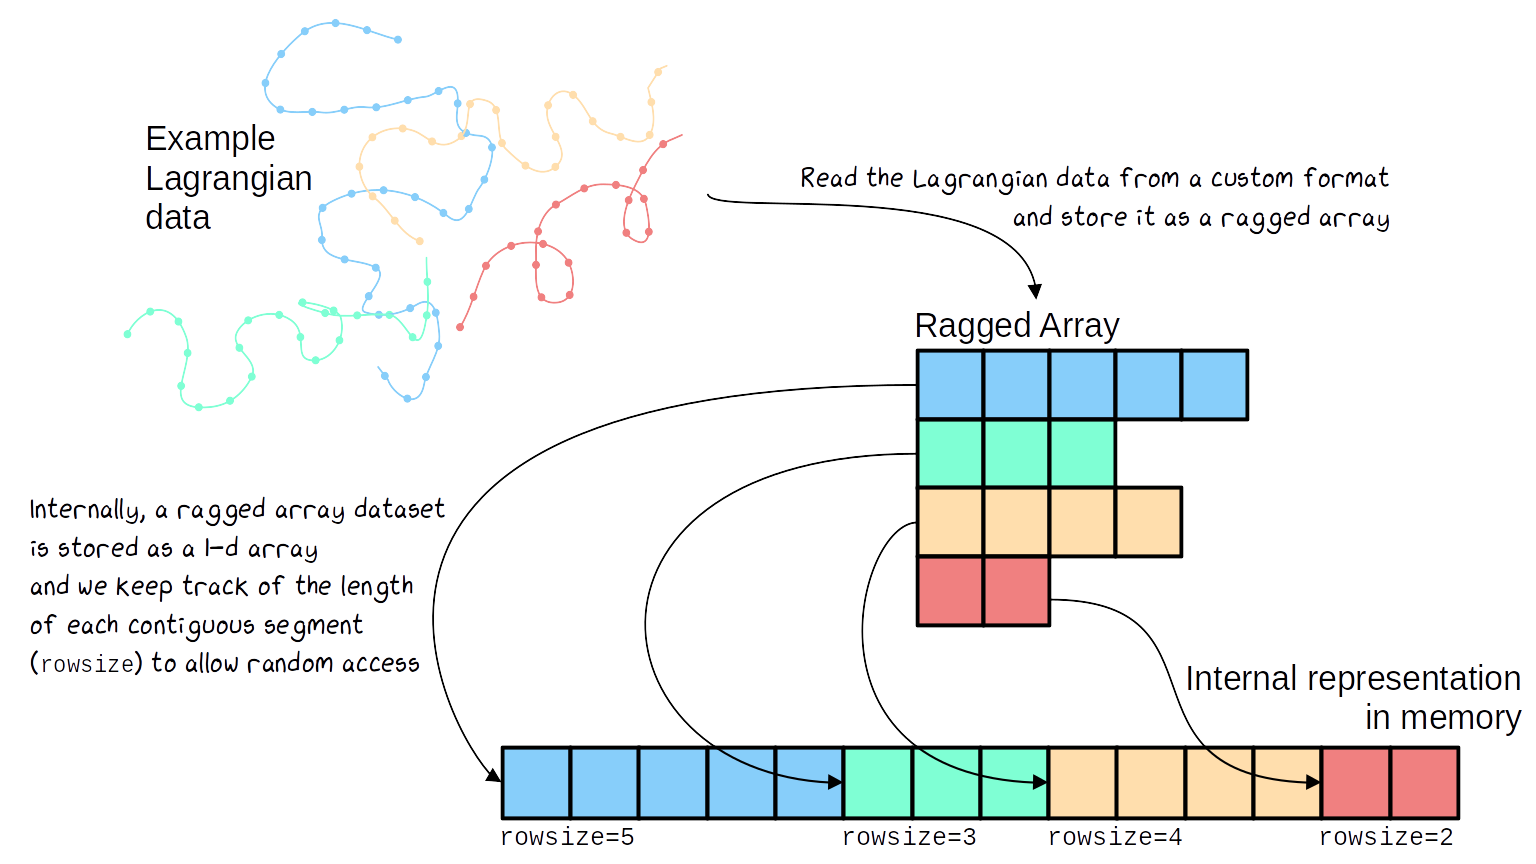
\includegraphics[width=0.5\linewidth]{ragged-array.png}
    
    \begin{itemize}
    \setlength\itemsep{0.1em}
        \item Clouddrift organizes data variables within a dataset in the Ragged Array data structure 
        \item A Ragged Array is organized where each \underline{particle/trajectory/row} associated observations are concatenated in order resulting in a 1-d array.
        \item A resulting metadata variable stores the rowsize of each individual \underline{particle/trajectory/row}.
    \end{itemize}
}

% footer
% generate qr code from https://www.qr-code-generator.com/ and replace qr_code.png
% default: barcode on the left
\makealtfooter{images/um-logo.png}{images/qr-code.png}

% replace with this like for barcode on the right
% \makealtfooter{images/qr-code.png}
 
\end{document}